\documentclass[rapport.tex]{subfiles}

\begin{document}
\section{Implementering}
	\subsection{Indledning}
	\subsection{Bruger-interface og applikation}
	I følgende afsnit vil implementeringen af bruger-interfacet og applikationen blive beskrevet. 
	\subsubsection{UserInterface}
	Biblioteker værd at nævne: Tkinter, Tkfiledialog\\
	
	Tkinter objekter er benyttet til at opbygge det grafisk brugerinterface som givet i design. 
	Hver knap er blevet oprettet med et tilknyttet funktionskald der udfører den ønskede funktion, som givet af de forskellige use cases. 
	Brugeren ser kun Tkinter objekter. 
	Knapperne til venstre i interfacet er sat i rækkefølge efter naturlig opsætning og eksekvering af real-time eye-tracking. Ikke tilgængelige funktioner har deaktiverede knapper således at man ikke kan foretage ulovlige handlinger. 
	Interaktion med andre klasser:
	For hver tilgang til præference-filen bliver der oprettet en ny instans af dataklassen SessionData fra klassen SessionHandler. Ved at aflæse indholdet/værdien af de forskellige Tkiner-objekter og skrive dette data til den instansen af SessionData, der senere bliver skrevet til præference-filen af klassen SessionHandler, vil der altid være konsistens mellem værdierne skrevet i brugerinterfacet, værdierne i præference-filen, og værdierne brugt i eye-tracking-algoritmen. 
	
	\begin{figure}
	\centering
	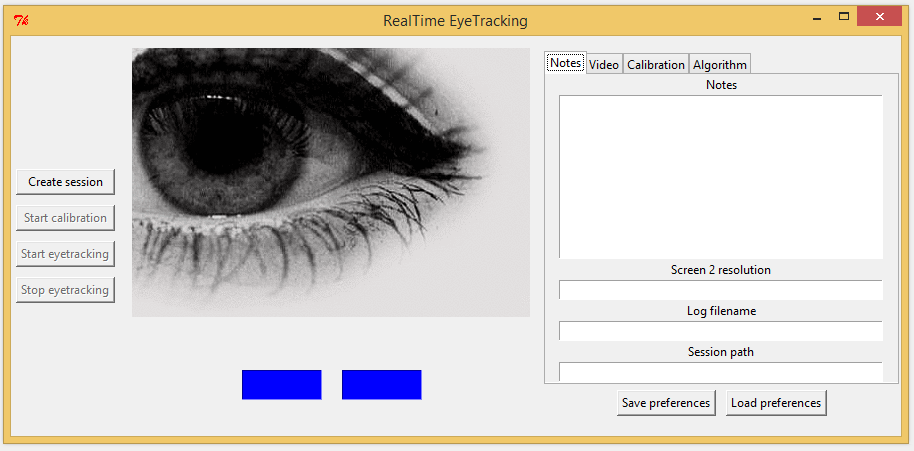
\includegraphics[width=0.7\linewidth]{GUI1}
	\caption{}
	\label{fig:GUI1}
	\end{figure}
	
	\subsubsection{SessionHandler}
	At nævne: Verificering af korrekt præference-fil. Vigtigheden og problemer med at have de forskellige værdier i strings (latin, utf8, ASCII). Bliver brugt som dataklasse
	Verificering fungerer ved at lede efter korrekt streng i hver linje. \\
	
\begin{lstlisting}
SESSIONPATH C:/RealTimeEyeTracking
USINGCAM True
CAMNR None
VIDEOPATH 0
NOTES Dette er en testsession
RESOLUTION 1600x900
CALTYPE Numbers
LOGFILENAME testlog
CALFILENAME testcallog
LOADEDCALDATA None
RECORDVIDEO False
RAWDATAPATH None
VARIABLENAMES['e_center', 'last_eyes', ...
VARIABLEVALUES['[0,0]', '[]', 'True', '20', '1500', ...
\end{lstlisting}
		
	\subsubsection{LogHandler}
	At nævne: StartTracking kører igennem her. Holder værdi om hvorvidt algoritmen kører. Bliver brugt som dataklasse. 
	Modtager en log-streng fra EyeTrackingHandler og gemmer den som angivet i SessionData dataklassen. 
	Vis eksempel på log-fil
	
	\subsubsection{CalibrationHandler}
	Vis eksempel på kalibrerings-fil
	
	\subsubsection{EyeTrackingHandler}
	
	
	\subsubsection{VideoCapture}
	Indeholder puplic funktion GetCameraInputs. 
	Andre funktioner er en del af klassen. Klassen oprettes med et video-input, og mulighed for kalibreringsdataet, samt ti frie variabler. Kalibreringsdataet og de ti frie variabler benyttes ikke til andet end at videresende til ETAlgorithm sammen med gyldig frame. 
	At passe kalibreringsdataet og de frie variabler igennem VideoCapture er ikke optimalt, men spiller ingen rolle i det samlede arbejdslæs. Det kan forestilles at man i stedet ville sende to pointers til hvor disse data ville være lageret. Argumentet for at passe disse data igennem VideoCapture er, at VideoCapture så vil kalde ETAlgorithm's Track() med den fundne frame samt disse data, i stedet for at returnere den fundne frame til EyeTrackingHandler og derefter kalde Track(). 
		

	\subsection{Starburst-algoritmen}
	\subsection{Optimering}
	
	\subsubsection{Fremtidige optimeringsmuligheder}
	Python understøtter multitrådning, hvilket giver mulighed for at køre flere instanser af eye-tracking-algoritmen sideløbende. Skriv mere om muligheder for multitrådning, og hvorfor det kan virke.
	\subsection{Diskussion}
		
\end{document}